\documentclass[reprint,preprintnumbers,showpacs,amsmath,twocolumn,showkeys,aps,prl]{revtex4-1}
\pdfoutput=1
\usepackage{amssymb}
\usepackage{amsbsy}
\usepackage{amsmath}
\usepackage{graphicx}
\usepackage{dcolumn}
\usepackage{bm}
\usepackage{natbib}
\usepackage{epsfig}
\usepackage{epstopdf}
\usepackage{dsfont}

\usepackage{hyperref}
\usepackage[usenames,dvipsnames]{xcolor}
\hypersetup{colorlinks, linkcolor={red},citecolor={blue}, urlcolor={MidnightBlue}}

\usepackage{pdfpages}
\begin{document}

%\title{Dynamical Localization in a Disordered System: Suppressing the Relaxation of a Random Quantum Magnet by Coherent Periodic Drive}

\title{The fate of dynamical many-body localization in the presence of disorder}

\author{Analabha Roy$^1$, and Arnab Das$^2$}
\email{arnab.das.physics@gmail.com}
\affiliation{$^1$ Saha Institute of Nuclear Physics, $1$/AF Bidhannagar, Kolkata-$700064$ \\
$^2$ Indian Association for the Cultivation of Science, $2$A \& $2$B Raja S. C. Mullick Road,
Kolkata - $700032$}

\begin{abstract}
Dynamical localization is one of the most startling manifestations of quantum interference, 
where the evolution of a simple system is frozen out under a suitably tuned coherent periodic drive.   
Here, we show that, although any randomness in the interactions of a many body system kills dynamical localization eventually, spectacular remnants survive even when the disorder is strong. We consider a disordered quantum Ising chain where the transverse magnetization relaxes exponentially with time with a decay time-scale $\tau$ due to random longitudinal interactions between the spins. We show that, under external periodic drive, this relaxation slows down ($\tau$ shoots up) by {\it orders of magnitude} as the ratio of the drive frequency $\omega$ and amplitude $h_{0}$ tends to certain specific values (the freezing condition). If $\omega$ is increased while maintaining the ratio $h_0/\omega$ at a fixed freezing value, then $\tau$ diverges exponentially with $\omega.$ The results can be easily extended 
for a larger family of disordered fermionic and bosonic systems. 

\end{abstract}
\maketitle

The dynamics of quantum systems driven out of equilibrium by coherent periodic drives has
remained an intriguing topic of interest from the early days of quantum mechanics (see, e.g., \cite{Sakurai}) 
to date
\cite{Andre-1,Andre-2,AAR-PRL,AAR-Generic,Arimondo-Rev,Gauge-1a,Gauge-1b,Gauge-2,Manisha-Amit-Diptiman-da,
Prosen-1,Bastidas,victor,Sthitadhi,Analabha1,Analabha2,AD-KS-DS-BKC,Kris-Freezing,Ashhab-Nori,Luca-Rigol,Anushya,
Arimondo-1,Arimondo-2,Bloch-Periodic,Shengstock,DMF-IISER-Exp,Kaitzer,Gopar}. 
One interesting and well-known phenomenon in this field, where repeated quantum interference results in a
scenario which is quite counter-intuitive and unexpected from the classical point of view, 
is that of dynamical freezing in a quantum system under a periodic drive.  
Illustrious examples include the localization of a single quantum particle for all time while being forced periodically  
in free space (dynamical localization \cite{Dunlap}), or in one of the two wells of a double-well potential 
modulated sinusoidally (coherent destruction of tunneling \cite{Hanggi}). In both cases, this happens due to the coherent suppression of tunneling. 

A many-body version of this phenomenon, dubbed as dynamical many-body 
freezing, has also been observed both theoretically 
\cite{AD-DQH,SB-AD-SDG,AD-RM,Russomanno,Anatoli-Periodic,Sei-Book} 
and experimentally \cite{DMF-IISER-Exp}. Dynamical many-body freezing, however, is a 
more drastic version of dynamical localization: in the latter only the tunneling term is 
renormalized to zero by the external drive, resulting in 
localization in real space, while in the former the entire many-body Hamiltonian - with all its mutually
non-commuting terms - vanishes \cite{AD-DQH}. This implies 
freezing of any arbitrary initial state in the Hilbert space, rather than freezing of initial 
states localized in real space only. Intuitively, such an unequivocal freezing of all degrees of freedom 
of a many-body system seems possible only under very special circumstances, where certain simplicities in the structure of the Hamiltonian allow for such large-scale destructive quantum interference. Here, we demonstrate that such dynamical 
many-body freezing can have strong manifestations even in a system where dynamics 
is induced by interactions which are totally random.

The plan of the paper is as follows. After introducing the system and the drive, we briefly
sketch the content of our analytical approach to the problem. Then we discuss our main 
results in that light. The precise condition of maximal freezing is obtained from this
analysis. We also go beyond that, using exact numerical results for large system-sizes, averaged
over several disorder realizations, and discuss further characteristics of the phenomenon. 
Finally conclude with an outlook.
%%%%%%%%%%%%%%%%%%%%%%%%%%%%%%%%%%%%%%%%%%%%%%%%%%%%%%%%%%%%%%%%%%%%%%%%%%%%%%%%
%%%%%%%%%%%%%%%%%%%%%%%%%%%%%%%%%%%%%%%%%%%%%%%%%%%%%%%%%%%%%%%%%%%%%%%%%%%%%%%%
\noindent
%{\it The Model and the Phenomenon }
Consider the following disordered one-dimensional Ising chain, subjected to a 
sinusoidal transverse field: 
\begin{equation}
H(t) = -\alpha J \sum_{i}^{L-1} J_i \sigma^{x}_{i}\sigma^{x}_{i+1}  
-\sum_{i}^{L} \left\{h_{0}\sin{(\omega t)} + \alpha h_i\right\} \sigma^{z}_{i}, 
\label{H_OBC}
\end{equation}
\noindent where $\sigma^{\alpha}$'s ($\alpha = x,y,z$) are components of Pauli spins, $J_{i}$'s and 
$h_{i}$ are respectively the (quenched) interactions and on-site fields - both drawn randomly 
from a uniform distribution between $\left(-1,+1\right).$
The transverse field is subjected to an external  drive of frequency $\omega$ (period $T = 2\pi/\omega$) 
and amplitude $h_{0}$ (we set $\hbar = 1$).  
%%%%%%%%%%%%%%%%%%%%%%%%%%%%%%%%%%%%%%%%%%%%%%%%%%%%%%%%%%%%%%%%%%%%%%%%%%%%%%%%%%%%%%%%%%	
%Note: Change 'hires.eps' to 'lowres.pdf' in figs for arxiv submission
%%%%%%%%%%%%%%%%%%%%%%%%%%%%%%%%%%%%%%%%%%%%%%%%%%%%%%%%%%%%%%%%%%%%%%%%%%%%%%%%%%%%%%%%%%	
\begin{figure*}[t]
\ 
\epsfig{file=fig1_hires.eps,width=0.95\linewidth}
\caption{
(Color Online) Dynamical Freezing without field disorder ($h_i=0$):  
{\bf (a)} Exponential relaxation of the expectation value of ${m^{z}}$ with time for different
values of the drive frequencies $\omega$. Unless otherwise indicated, the drive amplitude $h_{0}$ is fixed at $7.0$. 
For certain specific values of $\omega$ (e.g., $\omega=5.07,11.64$), the relaxation is 
tremendously slowed down. The relaxation in the 
absence of the drive is labeled separately for comparison. The inset compares a representative sample of the numerical data (shown as points) to the curves fitted to them using Eq.~\ref{Exp-decay-fit}.  
{\bf(b)} {\it $\tau$ vs $\omega$ for fixed $h_{0}$}: 
The sharp peaks indicate dramatic enhancements of $\tau$ for certain values of $\omega$. 
Three of the most prominent peaks are identified
as $P_{1-3}$. The values of $\omega$ at these peaks are $P_1\approx3.24$, $P_2\approx5.07$, 
and $P_3\approx11.64$. Those 
values are identified to be the ones for which the effective Hamiltonian $H_{\rm eff}$
(Eq.~\ref{eq:heff}) vanishes. The red dot pointed by the arrow-head represents the 
case in absence of the drive. 
{\bf (c)} {\it $\tau$ vs $\omega$ at fixed $\eta$}:
Comparison of enhancement of $\tau$ as $\omega$ is increased keeping $\eta = \frac{4h_{0}}{\omega}$ fixed 
for two cases - under the freezing condition ${\mathcal J}_{0}(\eta) = 0$ ($\eta \approx 2.4048$), and away from it 
${\mathcal J}_{0}(\eta) \approx 0.765$
($\eta = 1.0$) as marked in the Fig. 
Exponential enhancement of $\tau$ with $\omega$ is observed (numerical data fitted with the
$\tau(\omega)\bigr|_{{\mathcal J}_{0}(\eta)=0} =  \tau_{0} + \tau_{s}e^{{\omega}/{\omega_{s}}}$
form)  under the freezing condition, while no noticeable variation of $\tau$ is observed away from the
freezing condition. 
Results are for $L=100,$ averaged over $> 10^3$ 
disorder realizations of the bonds $J_i$.
The error-bars due to disorder-induced fluctuations are about the point size (see e.g., Fig. S1 of Suppl. Matt.),
and hence omitted (except for (c)) to avoid cluttering.}  
\label{mz-Rlx-tau}
\end{figure*}

\noindent
The Hamiltonian in Eq.~\ref{H_OBC}
can be mapped to the Hamiltonian~\cite{Lieb,Young-Random,Dziarmaga-Random},
\begin{multline}
H(t) = - \alpha J \sum_{i}^{L}  J_i \left(c^{\dagger}_i c^{\dagger}_{i+1} 
+ c^{\dagger}_i c_{i+1}  + {\rm h.c.}\right) \\
- 2 \sum_i^{L} \left\{h(t)+\alpha h_i\right\} c^{\dagger}_i c_i,
\label{H_Fermi}
\end{multline}
\noindent
with hard-core bosons  created (annihilated) by $c^\dagger_i$ ($c^{\;}_i$)
These bosons satisfy $\{ c_{j}^{\dagger},c_{j} \}=0$, and the usual bosonic commutation relations for $i\ne j$. Also, $h(t)=h_0\sin{\omega t}$.

In order to gain insight into the drive-dependent sharp jumps in the relaxation time-scale,
we follow a recently developed scheme \cite{Mintert} of deducing a renormalized time-independent effective 
Hamiltonian $H_{\rm eff}$ which describes the evolution of the system if observed stroboscopically at instants
$t = nT$, where $n$ denotes natural numbers: $U(nT) = e^{-iH_{\rm eff}nT},$ 
where $U(t) = {\mathcal T}\exp{[-i\int_{0}^{t}H(t^{\prime})dt^{\prime}]}$ (${\mathcal T}$ denotes time-ordering).  
For $\omega \gg |\alpha J|$, \textit{i.e.} in the limit of fast drive, no appreciable evolution takes place within a 
period, and stroboscopic observations represent smooth evolutions to a good approximation.  
It follows from Floquet theory~\cite{Floquet-Original} that for a $T$-periodic Hamiltonian $H(t),$ 
the time-evolution operator can be written as $U(t) = e^{-iH_{\rm eff}t}Z(t),$ where $Z(t)$ is $T$-periodic 
and $H_{\rm eff}$ is Hermitian. Clearly, $H_{\rm eff}$ is an operator that is largely non-local in the original 
degrees of freedom and is not necessarily amenable to any simple physical interpretation. 
However, since $Z(0)=Z(nT)=\mathds{1}$ (identity), $H_{\rm eff}$ can be considered as
an effective time-independent Hamiltonian giving the correct stroboscopic evolution. 
Using the above decomposition of $U(t)$ and the time-dependent Schr\"{o}dinger equation it satisfies, we get
\begin{equation} 
H_{\rm eff} = Z^{\dagger}(t)H(t)Z(t) -iZ^{\dagger}(t)(\partial_{t}Z(t)).
\label{Heff} 
\end{equation}
\noindent
Deducing the exact form of $H_{\rm eff}$ from the above equation is as hard as solving the original 
time-dependent problem. However, controlled approximations in the large $\omega$ limit can
be obtained \cite{Mintert} using a flow equation technique \cite{Wegner,Kehrein-book} 
which we employ here. This gives (see Suppl. Matt. for details)
\begin{multline}
\label{eq:heff}
H_{\rm eff}    =   -J\sum_i j^{(0)}_i\left(c^\dagger_i c^\dagger_{i+1} + \rm{h.c.}\right) \\
		            -J\sum_i j^{(1)}_i\left(c^\dagger_i c^{\;}_{i+1}+\rm{h.c}\right) 
		            -\mu\sum_i j^{(2)}_i c^\dagger_i c^{\;}_i,
\end{multline}
with $\eta \equiv 4h_0/\omega$, and the constants $j^{(s)}_i, \mu $ defined as follows.
\begin{eqnarray}
j^{(0)}_i            &\equiv& \alpha J_i\; \bigg\{\mathcal{J}_0(\eta) - \frac{4\alpha h_i}{\omega}\beta(\eta)\bigg\} ,\nonumber \\
j^{(1)}_i            &\equiv& \alpha J_i \; \mathcal{J}_0(\eta) ,\nonumber \\
j^{(2)}_i            &\equiv& \frac{h_i}{J},\nonumber \\
\mu 		     &\equiv& 2\alpha J.
\label{Renorm_fctr}
\end{eqnarray}
Here, $\mathcal{J}_0(\eta)$ is the ordinary Bessel function of order zero
(note that the way they are defined in Eq.~(\ref{H_OBC}), $J_{i}$s are 
dimensionless and $h_{i}$'s have dimension of energy). In addition, the function $\beta(\eta)\equiv\sum_{n\neq 0} {\mathcal{J}_n(\eta)}/{n}$. 

The above expression for $H_{\rm eff}$ is obtained under a rotating-wave approximation
(RWA) which holds for $\omega \gg J,\alpha.$ This effective Hamiltonian accurately reproduces the dynamics 
of the full system stroboscopically to the lowest order in $\alpha/\omega$~\cite{suppl}.
%%%%%%%%%%%%%%%%%%%%%%%%%%%%%%%%%%%%%%%%%%%%%%%%%%%%%%%%%%%%%%%%%%%%%%%%%%%%%%%%%%%%%%%%%%	
%Note: Change 'hires.eps' to 'lowres.pdf' in figs for arxiv submission
%%%%%%%%%%%%%%%%%%%%%%%%%%%%%%%%%%%%%%%%%%%%%%%%%%%%%%%%%%%%%%%%%%%%%%%%%%%%%%%%%%%%%%%%%%
\begin{figure}[htb]
\ 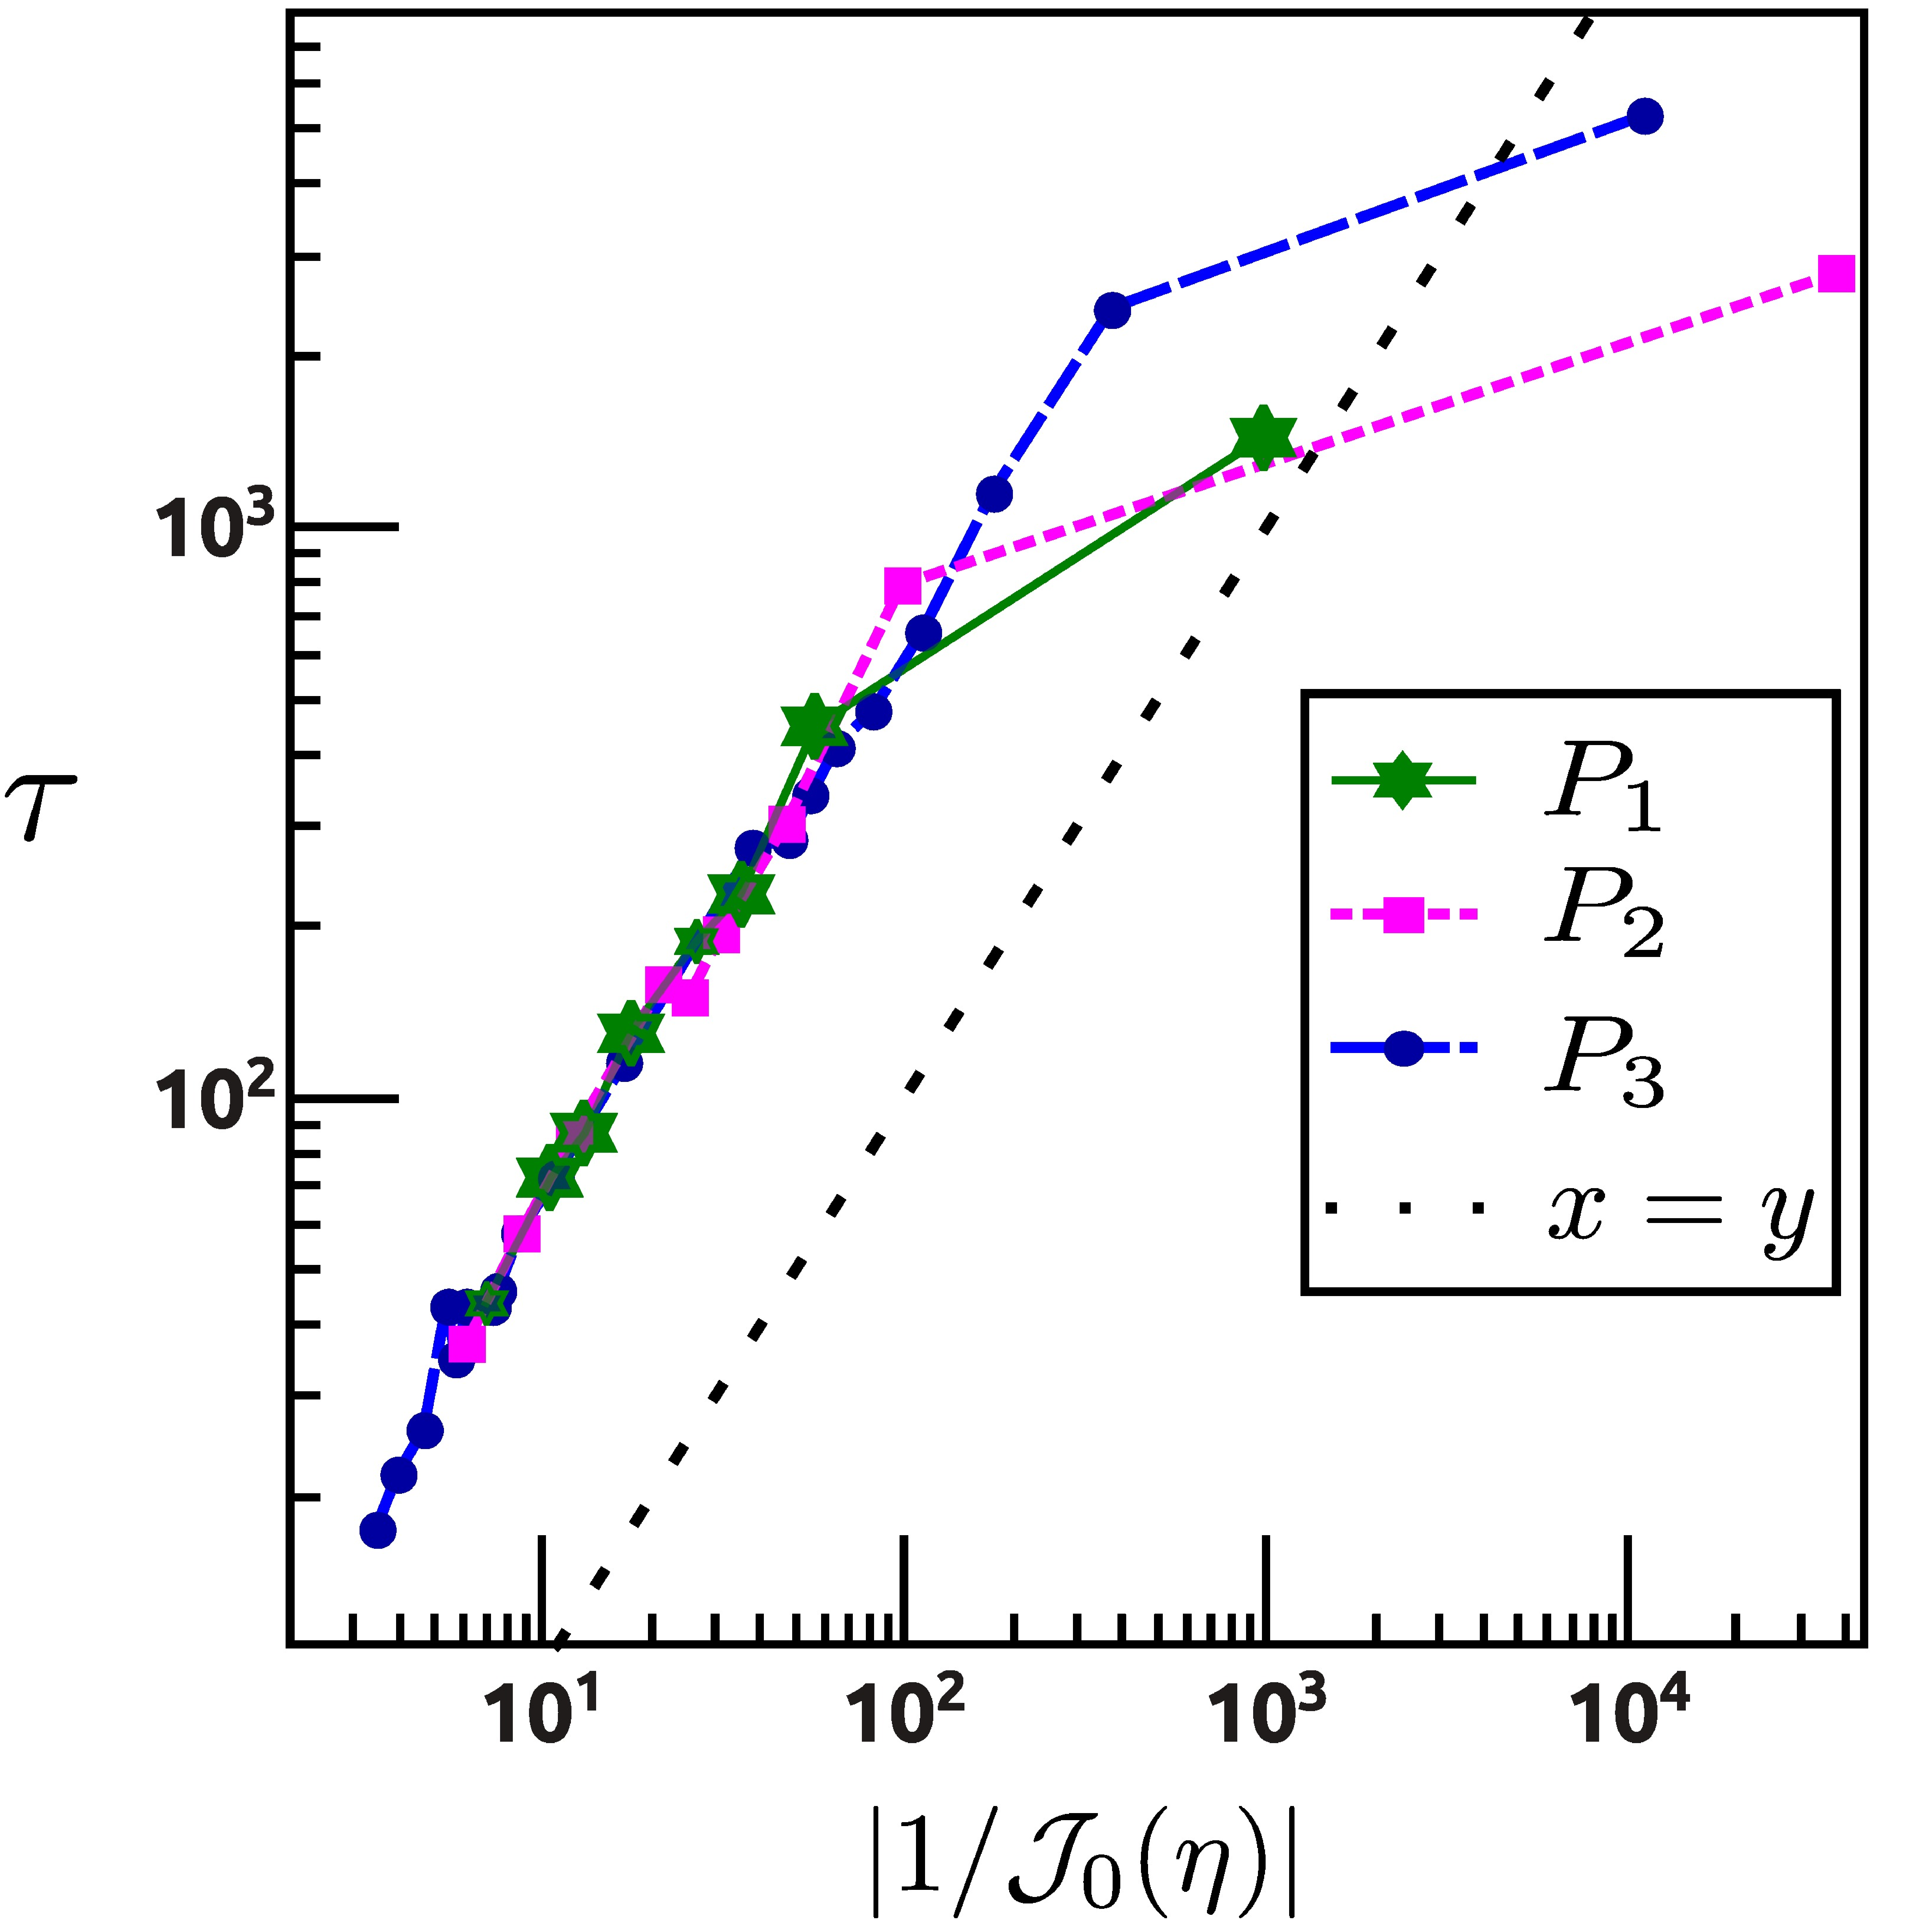
\epsfig{file=fig2_hires.eps,width=0.7\linewidth}
\caption{(Color Online) Dependence of $\tau$ on the drive parameters.
Numerical data for $\tau$ vs $1/{\mathcal J}_{0}(\eta)$ for $h_{i}=0$, $h_{0}=7$ 
(for a single random realization) are shown for the range of $\omega$ around the peaks $P_{1,2,3}$ 
of Fig.~\ref{mz-Rlx-tau}(b). The black dashed line is a guide to the eye. 
As expected from Eqs.~(\ref{eq:heff}, \ref{Renorm_fctr}),
we observe $\tau \propto 1/{\mathcal J}_{0}(\eta)$ where ${\mathcal J}_{0}(\eta) \gg  \alpha/\omega^{2}$.
However, for small ${\mathcal J}_{0}(\eta),$ $\tau$ tends to saturate to a large value \textit{viz.} the respective 
peak values in Fig.~\ref{mz-Rlx-tau}(b) (instead of diverging).}
\label{tau-vs-J0}
\end{figure}
%%%%%%%%%%%%%%%%%%%%%%%%%%%%%%%%%%%%%%%%%%%%%%%%%%%%%%%%%%%%%%%%%%%%%%%%%%%%%%%%%%%
Now we describe our main results for the driven spin Hamiltonian $H(t)$ 
and analyze it in light of the effective time-independent Hamiltonian $H_{\rm eff}$.
To avoid cluttering, the results presented in Fig.~\ref{mz-Rlx-tau} and the main discussion
are focused on the case where the field disorder is absent ($h_{i}=0$), the case with $h_{i}\ne 0$ is given afterwards.
Imagine that the spins (in $H(t)$) are initially prepared in a state strongly polarized in $+z$-direction 
and the transverse magnetization $ m^{z} = \frac{1}{L}\langle\sum_{i=1}^{L}\sigma_{i}^{z}\rangle \approx 1$. 
(here $\langle ... \rangle$ denotes quantum expectation values, 
and $\overline{{\mathcal O}}$ denotes average of ${\mathcal O}$ over disorder realizations).
In the absence of the drive ($h_{0}=0$), the magnetization $m^z$ relaxes with time since the random interaction terms in the Hamiltonian do not commute with it. If the drive is switched on, the characteristic time-scale of the relaxation 
changes, depending on the drive. The relaxations of $\overline{m^{z}}$ with time for various drive 
frequencies are shown in Fig.~\ref{mz-Rlx-tau}(a) (these results are obtained by numerically solving the 
time-dependent Schr\"{o}dinger equation for several disorder realizations and averaging 
over them). The relaxations (both in the absence and presence of the drive) 
are fitted accurately with the exponential decay form 
(inset of Fig.~\ref{mz-Rlx-tau}(a)).
\begin{equation}
\overline{\langle m^{z}(t)\rangle} =  m^{z}_{0}e^{-t/\tau},
\label{Exp-decay-fit}
\end{equation} 
\noindent
where $\tau$ is the decay constant. Our main result concerns the behavior of the decay time-scale $\tau$ 
as a function of the drive frequency $\omega$ for a given drive amplitude $h_{0}$. \\

\noindent
{\it Freezing Points:}
The behavior is quite dramatic, as shown in Fig.~\ref{mz-Rlx-tau}(b):
for certain values of $\omega$, the value of $\tau$ shoots up sharply 
by orders of magnitude compared to the undriven case. This corresponds 
to the extreme slowing down (freezing) of the decay of $m^z$ visible for certain 
values of $\omega$ in Fig.~\ref{mz-Rlx-tau}(a).
This can be explained by noting that for $h_{i}=0$ (as considered in the figure), 
the effective Hamiltonian  $H_{\rm eff} \propto {\mathcal J}_{0}(\eta)$ to leading order in $\alpha/\omega$ 
(Eq.~\ref{eq:heff},\ref{Renorm_fctr}) and hence $\tau \propto 1/{\mathcal J}_{0}(\eta)$ for $\omega \gg J,\alpha,$ (see Fig.~\ref{tau-vs-J0}). Thus, there is an overall renormalization of the time-scale, which can be controlled
by the factor ${\mathcal J}_{0}(\eta).$ Under the special condition ${\mathcal J}_{0}(\eta)=0$ (the freezing condition), $H_{\rm eff}$ 
vanishes, indicating a large enhancement of {\it all} timescales observable in the dynamics governed by $H_{\rm eff}$.
Interestingly, this implies that the slowing down is not only limited to $m^z(t)$, 
or to any special initial condition. 
For finite $\omega$, the approximation is, of course, valid only as long as 
${\mathcal J}_{0}(\eta) \gg \alpha/\omega^{2}$ -- otherwise higher order terms in $\alpha/\omega$ 
come into play. This results in a saturation due to the breakdown in the linear behaviour of $\tau$ with $1/{\mathcal J}_{0}(\eta)$ (Fig.~\ref{tau-vs-J0}). The saturation is also seen in the large but finite values of $\tau$ observed
at the freezing points ($P_{1,2,3}$) of Fig.~\ref{mz-Rlx-tau} (b), instead of infinite $\tau$ as suggested by 
the vanishing of $H_{\rm eff}$ at those points.    \\

\noindent{\it Beyond the Rotating-Wave Approximation:}
Though $\tau$ does not diverge for finite $\omega$ due to higher order corrections to 
RWA, those corrections should vanish as $\omega \to \infty,$ 
resulting in $\lim_{\omega\to\infty}\tau\to\infty$
under the freezing condition ${\mathcal J}_{0}(\eta)=0.$ To characterize the dependence of $\tau$ on $\omega$ 
under the freezing condition going beyond RWA, 
we numerically study the variation of $\tau$ with $\omega$ fixing $\eta$ to a freezing value. 
Fig.~\ref{mz-Rlx-tau} (c) shows that $\tau$  
diverges exponentially with $\omega$. The numerical results in the figure are  
fitted well with the form $\tau(\omega)\bigr|_{{\mathcal J}_{0}(\eta)=0} =  \tau_{s}e^{{\omega}/{\omega_{s}}}-\tau_0$. 
If $\eta$ is held fixed to some value such that ${\mathcal J}_{0}(\eta) \not\approx 0$ (away from freezing), $\tau$ does not show
any appreciable change with increase in $\omega$ within the range considered (Fig.~\ref{mz-Rlx-tau} c). In this range,
$\tau$ increased by orders of magnitude for the freezing case. \\

\noindent{\it The $\omega \to \infty$ limit:} 
Note that absolute 
freezing, \textit{i.e.} the divergence of $\tau$ in the $\omega \to \infty$ limit 
under the freezing condition, is a counter-intuitive result. Intuitively, an infinitely 
fast purely sinusoidal drive should simply be equivalent to the absence of the drive altogether, 
since the driven parameters return back to themselves within no appreciable time in each cycle. 
This would mean that $m^z$ should decay when $\omega \to \infty$ 
as if there was no drive at all. This is indeed the case away from freezing -- in the large $\omega$
range we considered, (see Fig~\ref{mz-Rlx-tau} c), $\tau$ remains same 
as that of the undriven case as $\omega$ is increased. However, 
under the freezing condition, $\tau$ diverges exponentially, indicating that the decay will completely
stop due to the drive as $\omega \to \infty$. \\
%%%%%%%%%%%%%%%%%%%%%%%%%%%%%%%%%%%%%%%%%%%%%%%%%%%%%%%%%%%%%%%%%%%%%%%%%%%%%%%%%%%%%%%%%%	
%Note: Change 'hires.eps' to 'lowres.pdf' in figs for arxiv submission
%%%%%%%%%%%%%%%%%%%%%%%%%%%%%%%%%%%%%%%%%%%%%%%%%%%%%%%%%%%%%%%%%%%%%%%%%%%%%%%%%%%%%%%%%%
\begin{figure*}[t]
\ 
\epsfig{file=fig3_hires.eps,width=0.7\linewidth}
\caption{
(Color Online) Dynamical Freezing with field disorder:  
{\bf (a)} Exponential relaxation of $m^{z}$ with time for different
values of the drive frequencies $\omega$. {\bf (b)} 
The timescale $\tau$ of the exponential relaxation of $m^z$ vs $\omega$. 
Note the peaks at the roots of $\mathcal{J}_0(\eta)$, the same places as peaks 
$P_{1-3}$ in Fig~\ref{mz-Rlx-tau}. The red dot pointed by the arrow-head represents 
the case in absence of the drive. The inset plots $\tau$ vs $\omega$ (log-scale) at 
smaller values while adjusting $h_0$ so as to remain at the first root of  $\mathcal{J}_0(\eta)$. 
At very small values of $\omega$, the higher order contributions destroy the dynamical 
equivalence between $H(t)$ and $H_{\rm eff}$, leading to a loss of freezing. 
Freezing begins to appear as $\omega$ is increased, as seen in the inset by the growth of $\tau$ with $\omega$
for $\eta$ fixed to a freezing value. All the parameters are the same 
as in Fig~\ref{mz-Rlx-tau}, except with field disorder $h_i$ switched on.
$h_{i}$ is distributed uniformly and randomly between $\pm 1$}. 
\label{mz-Rlx-tau-fdon}
\end{figure*}
%%%%%%%%%%%%%%%%%%%%%%%%%%%%%%%%%%%%%%%%%%%%%%%%%%%%%%%%

\noindent
{\it Static disordered field ($h_i\neq 0$):}
Now we briefly present the results for the case with quenched disorder in the transverse field.
Including randomness in the field does not alter the basic features of the phenomenon discussed above, 
but there are some quantitative differences that we discuss here. In this case $H_{\rm eff}$
does not vanish even to first order in $1/\omega$ at the freezing point due to the field-dependent 
terms in Eq.~\ref{eq:heff} that scale inversely with $\omega$. Thus, we expect freezing at the roots of 
$\mathcal{J}_0(\eta)$ to last for shorter times at large $\omega$ when the field 
disorder is on. This is qualitatively verified by our numerical simulations of the 
exact dynamics with field disorder on. Figure~\ref{mz-Rlx-tau-fdon} shows plots of $m^z$ and the 
exponential relaxation time scale therein in regimes similar to Fig.~\ref{mz-Rlx-tau}, except with 
the field disorder switched on. The plots show that freezing is maintained at the roots of 
$\mathcal{J}_0(\eta)$, although the time scale of the decay is one order of magnitude less than the 
case without any static field.

\noindent
{\it Summary and Outlook:}
We have shown that dynamical localization can have drastic manifestations in many-body systems with
extensive disorder. We show that the application of a coherent periodic drive with specific values of the ratio 
of the drive frequency $\omega$ and the amplitude $h_{0}$ (freezing condition), can drastically slow 
down the natural relaxation induced by random interactions between the spins in a disordered Ising chain
for {\it any arbitrary initial state in the Hilbert space}. 
For moderately high values of $\omega$ and $h_{0}$, $\tau$ is observed to be orders of magnitude higher 
than its value away from freezing (or that in absence of the drive). At a specific freezing point 
($h_{0}/\omega$ kept fixed), the characteristic relaxation time $\tau$ diverges exponentially with 
$\omega$. However, if the ratio is fixed away from the freezing value, increasing $\omega$
does not have any observable effect on $\tau.$ These results are the first of their kind, showing drastic survival of 
dynamical localization, which is the result of large-scale destructive quantum interference induced by a 
periodic drive, in a highly disordered system. This opens up possibilities of preserving arbitrary (even unknown) 
quantum states of interacting qubits (Ising spins) from decaying due to unknown stray interactions.   
Experimental realizations of bosons in disordered 1d potentials in optical lattices have already been achieved 
experimentally~\cite{Disordered-Bosons,Bloch-Nat-Phys}. Coherent periodic drives applied to hardcore bosons
in optical lattices, used for realizing spin chains with precise control over the Ising-like
couplings, have also materialized~\cite{Bloch-Periodic}.
Hence, experimental observations of the freezing phenomenon seem feasible 
in a present day cold-atom laboratory.       \\
\noindent
{\it Acknowledgements:}
AR thanks CSIR, India for support under Scientists' Pool Scheme No. $13(8531-$A$)/2011/$Pool, as well as the TACC, University 
of Texas at Austin, for access to their clusters. Both authors thank Kasturi Basu, IACS Kolkata, for useful discussions.

\bibliographystyle{apsrev4-1}
\bibliography{bib_freezing} 
 
%%%%%%%%%%%%%%%%%%%%%%%%%%%%%%%%%%%%%%%%%%%%%%%%%%%%%%%%%%%%%%%%%%%%%%%%%%%%%%%%%%%%%%%%%%	
%Note: Uncomment these for arxiv submission. Update PDF filename and add pages if needed
%%%%%%%%%%%%%%%%%%%%%%%%%%%%%%%%%%%%%%%%%%%%%%%%%%%%%%%%%%%%%%%%%%%%%%%%%%%%%%%%%%%%%%%%%%
%\clearpage \includepdf[pages=1]{DMF-Random_suppl.pdf}
%\clearpage \includepdf[pages=2]{DMF-Random_suppl.pdf}
%\clearpage \includepdf[pages=3]{DMF-Random_suppl.pdf}
%\clearpage \includepdf[pages=4]{DMF-Random_suppl.pdf}
%\clearpage \includepdf[pages=5]{DMF-Random_suppl.pdf}
%\clearpage \includepdf[pages=6]{DMF-Random_suppl.pdf}
%\clearpage \includepdf[pages=7]{DMF-Random_suppl.pdf}


\end{document}
